%----------------------------------------------------------------------------------------
%	PACKAGES AND OTHER DOCUMENT CONFIGURATIONS
%----------------------------------------------------------------------------------------

\documentclass[a4paper]{article}

\usepackage{amsmath}

\usepackage{mhchem}

\usepackage{gensymb}

%\usepackage[super]{natbib}

\usepackage[T1]{fontenc} % Use 8-bit encoding that has 256 glyphs

\usepackage{lmodern}

\usepackage[hyphenbreaks]{breakurl}

\usepackage[hyphens]{url}

%\usepackage[super,sort&compress]{natbib}
%\usepackage{natbib}
%\setlength{\bibsep}{0.0pt}

\usepackage{subcaption}

\usepackage{graphicx}

\linespread{1.05} % Line spacing - Palatino needs more space between lines
\usepackage{microtype} % Slightly tweak font spacing for aesthetics

\usepackage[spanish]{babel} % Language hyphenation and typographical rules

\usepackage[numbib,notlof,notlot,nottoc]{tocbibind} % Shows bibliography as a section

\usepackage[hmarginratio=1:1,top=32mm,columnsep=20pt]{geometry} % Document margins

\usepackage[section]{placeins}

\usepackage{float}

\usepackage{booktabs} % Horizontal rules in tables

\usepackage{enumitem} % Customized lists


\usepackage{abstract} % Allows abstract customization

\renewcommand{\abstractnamefont}{\normalfont\bfseries} % Set the "Abstract" text to bold

\usepackage{fancyhdr} % Headers and footers
\pagestyle{fancy} % All pages have headers and footers
\fancyhead{} % Blank out the default header
\fancyfoot{} % Blank out the default footer
\fancyhead[C]{Apuntes y ejercicios resueltos de Estructura de la Materia 2 $\bullet$ Ignacio Poggi} % Custom header text
\fancyfoot[C]{\thepage} % Custom footer text

\usepackage{titling} % Customizing the title section

\usepackage{hyperref} % For hyperlinks in the PDF

%----------------------------------------------------------------------------------------
%	TITLE SECTION
%----------------------------------------------------------------------------------------

\setlength{\droptitle}{-4\baselineskip} % Move the title up

\pretitle{\begin{center}\LARGE\bfseries} % Article title formatting
\posttitle{\end{center}} % Article title closing formatting
\title{Estructura de la Materia 2} % Article title
\author{%
\textsc{Ignacio Poggi} \\[1ex] % Your name
\normalsize \href{mailto:ignaciop.3@gmail.com}{ignaciop.3@gmail.com} % Your email address
}

\date{\today} % Leave empty to omit a date
\renewcommand{\maketitlehookd}{%
\begin{abstract}
\noindent Apuntes y ejercicios resueltos de Estructura de la Materia 2 (2º cuatrimestre 2022).
\end{abstract}
}

%----------------------------------------------------------------------------------------

\begin{document}
\maketitle

% Print the title

%----------------------------------------------------------------------------------------
%	ARTICLE CONTENTS
%----------------------------------------------------------------------------------------

\section{Gu\'ia 1: Redes Cristalinas y Espacio Rec\'iproco}

\subsection{}

\begin{itemize}
\item En este \'item nos piden describir una estructura c\'ubica centrada en la base (SC con puntos adicionales en las caras horizontales de la celda).

\begin{figure}[H]
  \centering
  \begin{subfigure}[b]{0.4\linewidth}
    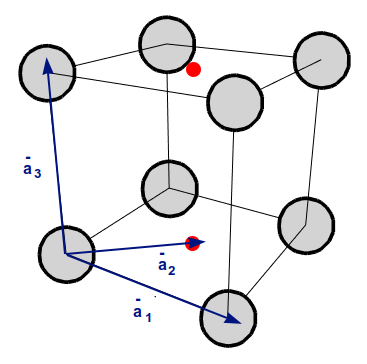
\includegraphics[width=\linewidth]{cubo3d_ej1.png}
     \caption{Red c\'ubica centrada en la base con una posible elecci\'on de vectores primitivos.}
  \end{subfigure}
  \begin{subfigure}[b]{0.4\linewidth}
    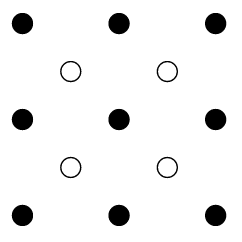
\includegraphics[width=\linewidth]{red_cubica.png}
    \caption{Vista cenital de la red peri\'odica.}
  \end{subfigure}
  \label{fig:cubo3d_ej1}
\end{figure}

Esta red puede pensarse como suma de planos con dos redes SC en dos dimensiones superpuestas, por lo tanto, es red de Bravais (de ahora en adelante, RB).

Una posible elecci\'on de vectores primitivos es la siguiente:

$$\begin{cases}
\vec{a}_{1} = a\hat{x} \\
\vec{a}_{2} = \frac{a}{2}(\hat{x} + \hat{y}) \\
\vec{a}_{3} = a\hat{z}
\end{cases}$$

\item Para la c\'ubica centrada en los lados (SC con puntos adicionales en las caras verticales de la celda), es an\'alogo al caso a), describiendo a los vectores primitivos de la siguiente manera:

\begin{figure}[H]
  \centering
  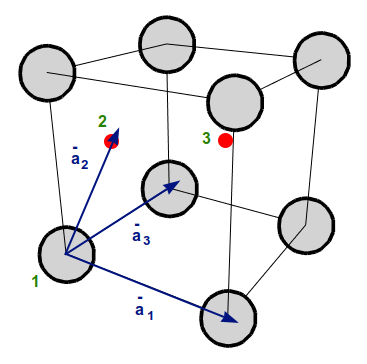
\includegraphics[width=0.5\linewidth,height=0.5\linewidth]{cubo3d_ej2.png}
  \caption{Red c\'ubica centrada en la base con una posible elecci\'on de vectores primitivos.}
  \label{fig:cubo3d_ej2}
\end{figure}

Observamos que no es una RB (como vemos en la figura (\ref{fig:cubo3d_ej2}) en color verde, desde el punto 2, vemos al punto 3; pero desde \'este no llegamos a 1). Podemos describir la red como una \textit{SC + base}:

$$base = \{ \vec{0}, \frac{a}{2}(\hat{z} + \hat{y}), \frac{a}{2}(\hat{x} + \hat{z})\}$$

\item Para la red c\'ubica centrada en las aristas, tenemos el mismo problema que la anterior (desde el punto 2 tengo al punto vecino 3; que no se ve desde 1 $\Rightarrow$ no es RB.

\begin{figure}[H]
  \centering
  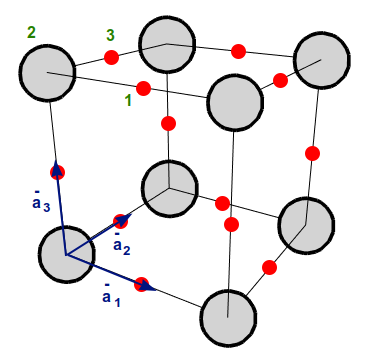
\includegraphics[width=0.5\linewidth,height=0.5\linewidth]{cubo3d_ej3.png}
  \caption{Red c\'ubica centrada en la base con una posible elecci\'on de vectores primitivos.}
  \label{fig:cubo3d_ej3}
\end{figure}

La describimos as\'i:

$$SC + base = SC + \{ \vec{0}, \frac{a}{2}\hat{x}, \frac{a}{2}\hat{y}, \frac{a}{2}\hat{z}\}$$

\end{itemize}

\subsection{}

\textbf{Red BCC (Body Centered Cube):}

\begin{figure}[H]
  \centering
  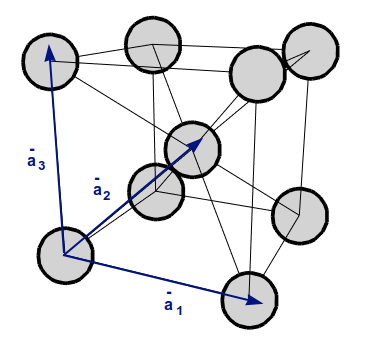
\includegraphics[width=0.5\linewidth,height=0.5\linewidth]{bcc.png}
  \caption{Red BCC con una posible elecci\'on de vectores primitivos.}
  \label{fig:bcc}
\end{figure}

Como vemos en la figura (\ref{fig:bcc}), uno de los posibles conjuntos de vectores primitivos para esta red es:

$$\begin{cases}
\vec{a}_{1} = a\hat{x} \\
\vec{a}_{2} = \frac{a}{2}(\hat{x} + \hat{y} + \hat{z}) \\
\vec{a}_{3} = a\hat{z}
\end{cases}$$

Otra elecci\'on:

$$\begin{cases}
\vec{a}_{1}' = a(\hat{x} + \hat{y}) \\
\vec{a}_{2}' = \frac{a}{2}(\hat{x} + \hat{y} + \hat{z}) \\
\vec{a}_{3}' = a(\hat{y} + \hat{z})
\end{cases}$$

Para hallar el volumen de la celda unidad, utilizamos la relaci\'on:

\begin{equation}
\label{eq:vol_celda_unidad}
V = | \vec{a}_{1} \cdot (\vec{a}_{2} \times \vec{a}_{3})|
\end{equation}

donde los $\vec{a}_{i}$ son los vectores primitivos. Entonces:

$$ \vec{a}_{2} \times \vec{a}_{3} = \begin{vmatrix}
\frac{a}{2} & \frac{a}{2} & \frac{a}{2} \\ 
0 & 0 & a
\end{vmatrix}  = (\frac{a^{2}}{2}, -\frac{a^{2}}{2}, 0) = \frac{a^{2}}{2}(\hat{x} - \hat{y})$$

$$ \Rightarrow \vec{a}_{1} \cdot (\vec{a}_{2} \times \vec{a}_{3}) = (a, 0, 0) \cdot (\frac{a^{2}}{2}, -\frac{a^{2}}{2}, 0) = \frac{a^{3}}{2}$$

$$ \Rightarrow V_{BCC} = | \vec{a}_{1} \cdot (\vec{a}_{2} \times \vec{a}_{3})| = |\frac{a^{3}}{2}| = \frac{a^{3}}{2}$$

Con la otra elecci\'on de vectores primitivos $\vec{a}_{i}'$, obtenemos el mismo resultado.\\

\textbf{Red FCC (Face Centered Cube):}

\begin{figure}[H]
  \centering
  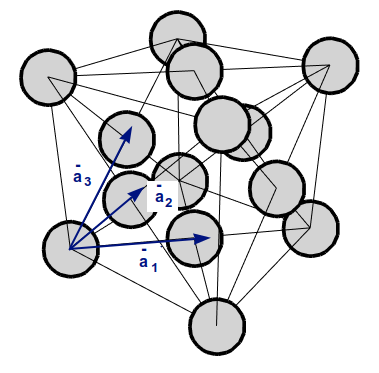
\includegraphics[width=0.5\linewidth,height=0.5\linewidth]{fcc.png}
  \caption{Red FCC con una posible elecci\'on de vectores primitivos.}
  \label{fig:fcc}
\end{figure}

Observamos en la a figura (\ref{fig:fcc}), los vectores primitivos para esta red:

$$\begin{cases}
\vec{a}_{1} = \frac{a}{2}(\hat{x} + \hat{y}) \\
\vec{a}_{2} = \frac{a}{2}(\hat{x} + \hat{z}) \\
\vec{a}_{3} = \frac{a}{2}(\hat{y} + \hat{z})
\end{cases}$$

Una elecci\'on m\'as turbia ser\'ia:

$$\begin{cases}
\vec{a}_{1}' = \frac{a}{2}(\hat{x} + \hat{y}) - a\hat{z} \\
\vec{a}_{2}' = a\hat{x} + \frac{a}{2}(\hat{y} + \hat{z}) \\
\vec{a}_{3}' = a\hat{z}
\end{cases}$$

Luego:

$$ \vec{a}_{2} \times \vec{a}_{3} = \begin{vmatrix}
\frac{a}{2} & 0 & \frac{a}{2} \\ 
0 & \frac{a}{2} & \frac{a}{2}
\end{vmatrix}  = (-\frac{a^{2}}{4}, -\frac{a^{2}}{4}, \frac{a^{2}}{4}) = \frac{a^{2}}{4}(- \hat{x} - \hat{y} + \hat{z})$$

$$ \Rightarrow \vec{a}_{1} \cdot (\vec{a}_{2} \times \vec{a}_{3}) = (\frac{a}{2}, \frac{a}{2}, 0) \cdot (-\frac{a^{2}}{4}, -\frac{a^{2}}{4}, \frac{a^{2}}{4}) = -\frac{a^{3}}{4}$$

Aplicamos (\ref{eq:vol_celda_unidad}) para hallar el volumen de esta celda:

$$ \Rightarrow V_{FCC} = | \vec{a}_{1} \cdot (\vec{a}_{2} \times \vec{a}_{3})| = |-\frac{a^{3}}{4}| = \frac{a^{3}}{4}$$

\subsection{}

Los primeros vecinos, por definici\'on, son todos aquellos que est\'an a distancia m\'inima de un elemento de la red. Se denomina \textbf{n\'umero de coordinaci\'on} al numero total de \'estos.\\

Los segundos y terceros vecinos son los que le siguen en distancia, respectivamente.\\

\textbf{Red c\'ubica simple:}\\

Para identificar m\'as f\'acilmente a los vecinos, ve\'amosla en 2D (teniendo en cuenta que la figura se repite en $\pm \hat{z}$, hac\'ia afuera/dentro de la hoja):

\begin{figure}[H]
  \centering
  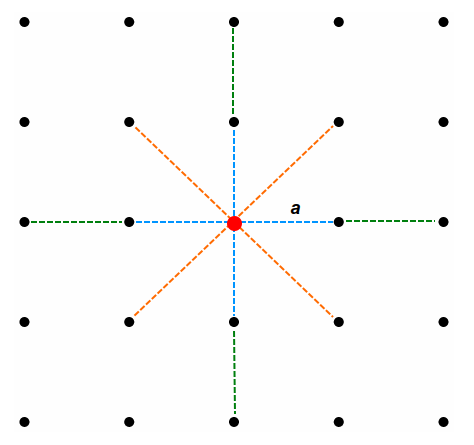
\includegraphics[width=0.5\linewidth,height=0.5\linewidth]{red2d_sc.png}
  \caption{Plano $xy$ de la red c\'ubica. Las l\'ineas azules marcan la distancia a primeros vecinos, las naranjas a segundos vecinos; y las verdes a terceros vecinos. El par\'ametro de red es $a$.}
  \label{fig:red2d_sc}
\end{figure}
 
Simplemente contamos los puntos y calculamos las respectivas distancias al elemento elegido (rojo):

\begin{center}
\# primeros vecinos = 6 (4 en el plano $xy$, 1 en $+\hat{z}$ y 1 en $-\hat{z}$) $\Rightarrow d = a$ \\
\# segundos vecinos = 12 (4 en el plano $xy$, 4 en $+\hat{z}$ y 4 en $-\hat{z}$) $\Rightarrow d = \sqrt{2a}$ \\
\# terceros vecinos = 8 (4 en $+\hat{z}$ y 4 en $-\hat{z}$) $\Rightarrow d = \sqrt{3a}$ \\
\end{center}

En 3D:

\begin{figure}[H]
  \centering
  \begin{subfigure}[b]{0.4\linewidth}
    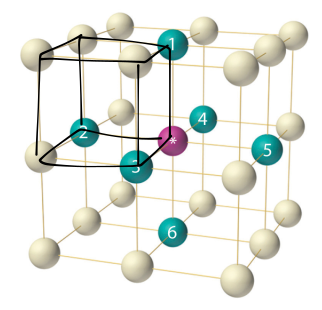
\includegraphics[width=\linewidth]{red3d_sc0.png}
     \caption{Primeros vecinos en color verde.}
  \end{subfigure}
  \begin{subfigure}[b]{0.4\linewidth}
    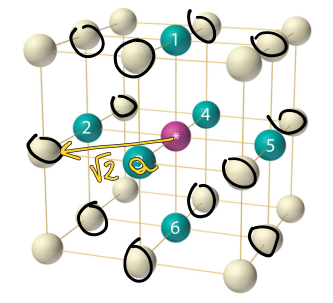
\includegraphics[width=\linewidth]{red3d_sc1.png}
    \caption{Segundos vecinos marcados en negro.}
  \end{subfigure}
  \begin{subfigure}[b]{0.4\linewidth}
    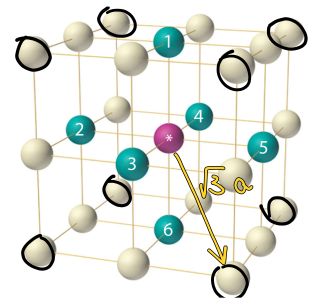
\includegraphics[width=\linewidth]{red3d_sc2.png}
    \caption{Terceros vecinos marcados en negro.}
  \end{subfigure}
  \caption{Primeros, segundos y terceros vecinos de una red SC tridimensional.}
  \label{fig:red3d_Sc}
\end{figure}

\textbf{Red BCC:}\\

\begin{figure}[H]
  \centering
  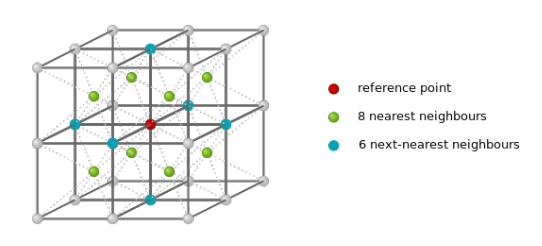
\includegraphics[width=0.7\linewidth,height=0.3\linewidth]{red3d_bcc.png}
  \caption{Primeros, segundos y terceros vecinos de una red BCC tridimensional.}
  \label{fig:red3d_bcc}
\end{figure}

\textbf{Red FCC:}\\

\begin{figure}[H]
  \centering
  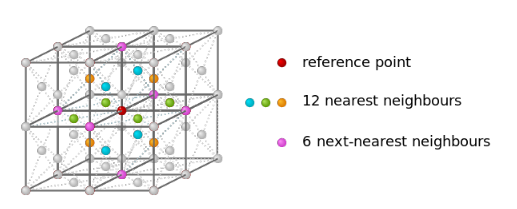
\includegraphics[width=0.7\linewidth,height=0.3\linewidth]{red3d_fcc.png}
  \caption{Primeros, segundos y terceros vecinos de una red FCC tridimensional.}
  \label{fig:red3d_fcc}
\end{figure}

\subsection{}

La fracci\'on de empaquetamiento es la relaci \'on entre el volumen de las esferas (\'atomos) y el volumen de la celda unidad:

\begin{equation}
\label{eq:empaq}
\rho_{X} = \frac{\frac{4}{3}\pi r^{3}}{V_{X}}
\end{equation}

donde

$$r = \frac{d_{1^{o} vecinos}}{2}$$

En la siguiente figura se observan las distribuciones aproximadas para cada red pedida:

\begin{figure}[H]
  \centering
  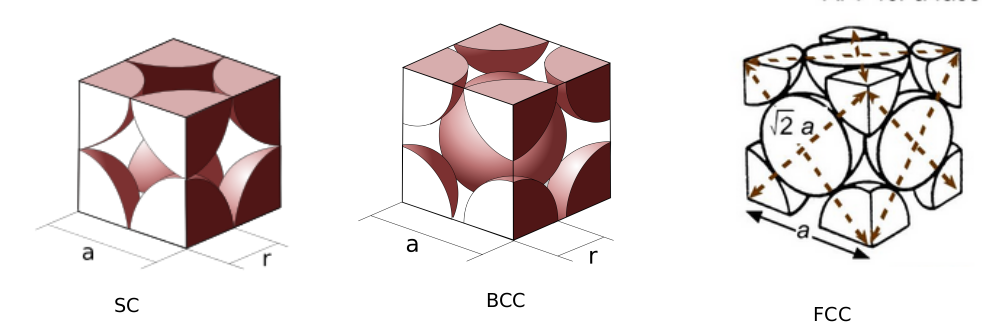
\includegraphics[width=0.9\linewidth,height=0.5\linewidth]{empaq.png}
  \caption{Empaquetamientos de las redes SC, BCC y FCC.}
  \label{fig:empaq}
\end{figure}

Aplicamos la ecuaci\'on (\ref{eq:empaq}) a cada red, con los datos de las distancias a primeros vecinos y volumen de cada celda unidad obtenidos en el ejercicio anterior, entonces:

$$ \rho_{SC} = \frac{\frac{4}{3}\pi r^{3}}{V_{SC}} = \frac{\frac{4}{3}\pi (\frac{a}{2})^{3}}{a^{3}} = \frac{\pi}{6} \approx 0.52$$

Esto quiere decir que, aproximadamente, el 52\% de la celda unidad SC est\'a ocupada por \'atomos.

$$ \rho_{BCC} = \frac{\frac{4}{3}\pi r^{3}}{V_{BCC}} = \frac{\frac{4}{3}\pi (\frac{\sqrt{3}}{4}a)^{3}}{\frac{a^{3}}{2}} = \frac{\sqrt{3}}{8}\pi \approx 0.68$$

$$ \rho_{FCC} = \frac{\frac{4}{3}\pi r^{3}}{V_{FCC}} = \frac{\frac{4}{3}\pi (\frac{\sqrt{3}}{2}a)^{3}}{\frac{a^{3}}{4}} = \frac{\sqrt{2}}{6}\pi \approx 0.74$$

Para la red diamante, veamos un esquema para orientarnos un poco mejor:

\begin{figure}[H]
  \centering
  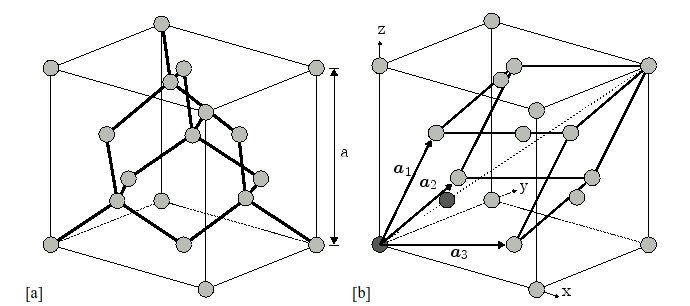
\includegraphics[width=0.9\linewidth,height=0.5\linewidth]{red3d_diamante.png}
  \caption{(a) Celda unidad de la estructura de diamante. (b) Se resaltan los vectores primitivos de una FCC, m\'as los dos \'atomos que conforman la base.}
  \label{fig:red3d_diamante}
\end{figure}

Esta red puede pensarse como dos FCC intercaladas, desplazadas una de la otra sobre la diagonal en $\frac{a}{4}(1, 1, 1)$.\\

Podemos hacer la siguiente elecci\'on para los vectores primitivos:

$$\begin{cases}
\vec{a}_{1} = \frac{a}{2}(\hat{y} + \hat{z}) \\
\vec{a}_{2} = \frac{a}{2}(\hat{x} + \hat{z}) \\
\vec{a}_{3} = \frac{a}{2}(\hat{x} + \hat{y})
\end{cases}$$

Entonces:

$$ Diamante = FCC + \{ \vec{0}, \frac{a}{4}(\hat{x} + \hat{y} + \hat{z})\}$$

Finalmente, calculemos su fracci\'on de empaquetamiento:

$$ \rho_{DIAMANTE} = \frac{\frac{4}{3}\pi r^{3}}{V_{DIAMANTE}} = \frac{\frac{4}{3}\pi (\frac{\sqrt{3}}{8}a)^{3}}{\frac{a^{3}}{4}} = \frac{\sqrt{3}^{3}}{96}\pi \approx 0.17$$

\subsection{}


%----------------------------------------------------------------------------------------
%	REFERENCE LIST
%----------------------------------------------------------------------------------------
\newpage
\begin{thebibliography}{99} % Bibliography - this is intentionally simple in this template
 
\end{thebibliography}


%----------------------------------------------------------------------------------------

\end{document}